% Paper III -- Nature Astronomy Article format (article class stand-in: no
% Nature class is installed; the structure, budgets and display-item count
% follow the journal's Article guide and are enforced by check_structure.py).
% Every number in this file comes from numbers.tex, which latex_tables.py
% generates from paper3/FROZEN.json; a line that must carry a literal
% (a definition, a literature value) ends with "% literal-ok".
\documentclass[11pt]{article}
\usepackage[a4paper,margin=25mm]{geometry}
\usepackage[T1]{fontenc}
\usepackage{amsmath,amssymb}
\usepackage{graphicx}
\usepackage{booktabs}
\usepackage{xspace}
\usepackage{xcolor}
\usepackage[numbers,sort&compress]{natbib}
\usepackage[colorlinks=true,linkcolor=blue!50!black,citecolor=blue!50!black,urlcolor=blue!50!black]{hyperref}
\graphicspath{{figures/}}
% generated by docs/paper3/latex_tables.py from paper3/FROZEN.json -- do not edit
% every number the manuscript quotes; rounding happens here only
\newcommand{\nPoints}{27\xspace}
\newcommand{\GateTwoCB}{27\xspace}
\newcommand{\GateTwoMedianR}{0.83\xspace}
\newcommand{\GateTwoMedianChi}{118\xspace}
\newcommand{\GateTwoBinnedCB}{27\xspace}
\newcommand{\TOneCB}{16\xspace}
\newcommand{\TOneCBXlow}{1 of 9\xspace}
\newcommand{\TOneCBXmid}{6 of 9\xspace}
\newcommand{\TOneCBXhigh}{9 of 9\xspace}
\newcommand{\TOneMedianChi}{25\xspace}
\newcommand{\TOneLeftover}{25\xspace}
\newcommand{\TOneDetermined}{27\xspace}
\newcommand{\TOneALMedian}{0.9\xspace}
\newcommand{\TOneALMax}{6.5\xspace}
\newcommand{\TTwoCB}{15\xspace}
\newcommand{\TTwoCBXlow}{4 of 9\xspace}
\newcommand{\TTwoCBXmid}{5 of 9\xspace}
\newcommand{\TTwoCBXhigh}{6 of 8\xspace}
\newcommand{\TTwoMedianChi}{22\xspace}
\newcommand{\TTwoLeftover}{24\xspace}
\newcommand{\TTwoDetermined}{26\xspace}
\newcommand{\TTwoDlnT}{0.28\xspace}
\newcommand{\TThreeCB}{10\xspace}
\newcommand{\TThreeCBXlow}{4 of 9\xspace}
\newcommand{\TThreeCBXmid}{3 of 9\xspace}
\newcommand{\TThreeCBXhigh}{3 of 8\xspace}
\newcommand{\TThreeMedianChi}{14\xspace}
\newcommand{\TThreeLeftover}{24\xspace}
\newcommand{\TThreeDetermined}{26\xspace}
\newcommand{\TThreeUnderdetermined}{1\xspace}
\newcommand{\TThreeBeyondLinear}{16 of 18\xspace}
\newcommand{\ControlCC}{21\xspace}
\newcommand{\ControlN}{27\xspace}
\newcommand{\BOpacityCB}{27\xspace}
\newcommand{\ThrChi}{4\xspace}
\newcommand{\ThrR}{0.3\xspace}
\newcommand{\ThrSignif}{3\xspace}
\newcommand{\nModels}{27\xspace}
\newcommand{\nCells}{162\xspace}
\newcommand{\nCellsRan}{162\xspace}
\newcommand{\nRedone}{9\xspace}
\newcommand{\WorstColourRange}{0.96--2.84\xspace}
\newcommand{\WorstColourRangeCoarse}{1.0--2.8\xspace}
\newcommand{\HeadlineColourRange}{1--3\xspace}
\newcommand{\gDmRange}{$-2.1$ to $-0.2$\xspace}
\newcommand{\gN}{102\xspace}
\newcommand{\KDmMax}{3.6\xspace}
\newcommand{\KN}{106\xspace}
\newcommand{\NIRNegative}{195 of 199\xspace}
\newcommand{\FloorNWell}{62\xspace}
\newcommand{\FloorNMin}{$10^{5}$\xspace}
\newcommand{\FloorMedian}{0.021\xspace}
\newcommand{\FloorNinety}{0.044\xspace}
\newcommand{\FloorMax}{0.18\xspace}
\newcommand{\FloorRedoneRange}{0.13--0.53\xspace}
\newcommand{\Distance}{40\xspace}
\newcommand{\DenseSurvives}{26\xspace}
\newcommand{\DenseEligible}{26\xspace}
\newcommand{\SparseSurvives}{18\xspace}
\newcommand{\SparseEligible}{18\xspace}
\newcommand{\OpticalSurvives}{25\xspace}
\newcommand{\OpticalEligible}{25\xspace}
\newcommand{\DenseTOne}{18\xspace}
\newcommand{\DenseTOneXlow}{2 of 9\xspace}
\newcommand{\DenseTOneXmid}{8 of 9\xspace}
\newcommand{\DenseTOneXhigh}{8 of 8\xspace}
\newcommand{\DenseTTwo}{14\xspace}
\newcommand{\DenseTThree}{10\xspace}
\newcommand{\SparseTOne}{5\xspace}
\newcommand{\SparseTOneEligible}{12\xspace}
\newcommand{\OpticalTOne}{2\xspace}
\newcommand{\OpticalTOneEligible}{25\xspace}
\newcommand{\DenseNIRShare}{33\%\xspace}
\newcommand{\IllumCos}{0.34\xspace}
\newcommand{\IllumNorm}{0.06\xspace}
\newcommand{\GasCos}{0.92\xspace}
\newcommand{\GasNorm}{1.35\xspace}
\newcommand{\ChainCells}{4\xspace}
\newcommand{\ChainBase}{2000\xspace}
\newcommand{\ChainTop}{8000\xspace}
\newcommand{\ChainTrapped}{10.5--13.8\%\xspace}
\newcommand{\ChainTrappedTop}{2.8--3.2\%\xspace}
\newcommand{\ChainDmChange}{0.14--0.21\xspace}
\newcommand{\ChainDmRefChange}{0.14--0.21\xspace}
\newcommand{\ChainSigns}{12 of 12\xspace}
\newcommand{\ChainCriterion}{4 of 12\xspace}
\newcommand{\ChainRelMax}{25\%\xspace}
\newcommand{\ChainBinnedSigns}{11 of 12\xspace}
\newcommand{\ChainBinnedCriterion}{5 of 12\xspace}
\newcommand{\ChainCB}{27\xspace}
\newcommand{\ChainN}{27\xspace}
\newcommand{\ChainMedianChi}{116\xspace}
\newcommand{\ChainMedianR}{0.83\xspace}
\newcommand{\SysLive}{524\xspace}
\newcommand{\SysKeys}{38\xspace}
\newcommand{\SysGtHalf}{56\%\xspace}
\newcommand{\SysGtHalfCount}{292 of 524\xspace}
\newcommand{\SysGtOne}{18\%\xspace}
\newcommand{\SysGtOneCount}{94 of 524\xspace}
\newcommand{\SysBinnedGtHalf}{60\%\xspace}
\newcommand{\SysBinnedGtOne}{22\%\xspace}
\newcommand{\SysControlGtHalf}{0\%\xspace}
\newcommand{\SysSign}{39 of 39\xspace}
\newcommand{\SysBinnedSign}{38 of 39\xspace}
\newcommand{\SysControlSign}{12 of 39\xspace}
\newcommand{\SysOneMode}{0.80\xspace}
\newcommand{\SysBinnedOneMode}{0.77\xspace}
\newcommand{\SysControlOneMode}{0.31\xspace}
\newcommand{\SysSVD}{0.82\xspace}
\newcommand{\SysSVDKeys}{24\xspace}
\newcommand{\SysNullMedian}{0.33\xspace}
\newcommand{\SysNullNinetyFive}{0.36\xspace}
\newcommand{\SysMPScale}{0.16\xspace}
\newcommand{\SysChiOne}{0.56\xspace}
\newcommand{\SysChiOneRange}{0.12--1.74\xspace}
\newcommand{\SysChiHalf}{2.3\xspace}
\newcommand{\SysBinnedChiOne}{0.67\xspace}
\newcommand{\SysControlChiOne}{0.002\xspace}
\newcommand{\SysResidOneMode}{0.76\xspace}
\newcommand{\SysResidGtHalf}{10\%\xspace}
\newcommand{\SysResidChiOne}{0.11\xspace}

\newcommand{\todo}[1]{\textcolor{red}{[TODO: #1]}}
\newcommand{\Cboth}{C\xspace}
\newcommand{\Cbin}{C$_{\rm bin}$\xspace}
\newcommand{\Aleg}{A\xspace}
\newcommand{\Bleg}{B\xspace}
\newcommand{\dRT}{d_{\rm RT}}
\newcommand{\Xlan}{X_{\rm lan}}
\newcommand{\Mej}{M_{\rm ej}}
\newcommand{\vej}{v_{\rm ej}}
\newcommand{\Teff}{T_{\rm eff}}
\newcommand{\Tgas}{T_{\rm gas}}
\newcommand{\chires}{\chi^2_{\rm res}/{\rm dof}}
\newcommand{\Rij}{R_{ij}}
\newcommand{\Msun}{M_\odot}
\newcommand{\LaII}{La\,\textsc{ii}\xspace}
\newcommand{\CeII}{Ce\,\textsc{ii}\xspace}
\newcommand{\PrII}{Pr\,\textsc{ii}\xspace}
\newcommand{\NdII}{Nd\,\textsc{ii}\xspace}
\newcommand{\sigsys}{\sigma_{\rm sys}}
\setlength{\parskip}{2pt}

\title{Coarse-grained line opacity leaves a detectable chromatic signature in kilonovae that ejecta parameters cannot mimic}
\author{Yonglin Zhu\\[2pt]
  \small \todo{affiliation}\\
  \small \texttt{zhuygln@gmail.com}}
\date{}

\begin{document}
\maketitle

\begin{abstract}
% six beats: problem; positive result; negative result; inference result;
% observational significance; physical interpretation.
Kilonova spectra are shaped by millions of lanthanide lines, which every model coarse-grains twice: the opacity is binned into an expansion opacity, and the redistribution of absorbed photons is reduced to a few-parameter rule. We test both approximations in one Monte Carlo code against a line-by-line fluorescence reference for heating-powered kilonovae with four lanthanide ions. Compressing the redistribution into a grouped kernel changes the photometry by less than the Monte Carlo noise. Coarse-graining the opacity makes every model too blue, by \HeadlineColourRange\ mag in colour, coherently across a \nPoints-point grid in ejecta mass, velocity and lanthanide fraction. No combination of those parameters reproduces the bias, and in lanthanide-rich ejecta neither does a free luminosity history; the residual remains detectable with standard optical and near-infrared follow-up at \Distance\ Mpc. Bolometric agreement between codes does not certify their colours: the opacity closure, not the redistribution closure, is the approximation that needs repair.
\end{abstract}

\section{Introduction}\label{sec:intro}

The kilonova that accompanied GW170817 was identified, and its ejecta weighed, through its colours: a blue optical transient fading within days and a red near-infrared one persisting for weeks \cite{gw170817,tanvir2017,chornock2017,kasen2017,metzger2020}. The inference from colour to composition runs through radiative transfer in an ejecta whose opacity is carried by tens of millions of lanthanide and actinide lines \cite{tanaka2020,kato2024,fontes2020,banerjee2022}. No code transports those lines one by one in a multidimensional, time-dependent calculation, and none needs to if two approximations hold. The first is the expansion opacity \cite{karp1977,eastman1993}: in homologous flow a photon sweeps through lines in frequency order, and the lines inside a velocity bin can be replaced by one continuous absorber. The second is a closure for what happens after absorption: a fluorescence cascade through the ion's level structure, replaced in practice by a two-level atom, a thermal re-emission, or a fixed redistribution rule \cite{lucy2002,lucy2003,sedona,tardis}. The two approximations are usually taken together and named after one of them---``the Sobolev expansion-opacity treatment''---so that a test of the pair cannot say which part failed.

Our companion papers separate them. The first (Paper~I) showed that the Sobolev line-by-line transfer and the expansion opacity are different approximations of the same forest and that only the second carries a density-dependent error \cite{sobolev1960,castor1970,jeffery1993}. The second (Paper~II) showed that line identity---which line a photon leaves through after it has been absorbed---is the physical content the two-level atom discards, and built a same-code Monte Carlo in which the fluorescence reference and its closures run on identical atoms, packets and boundaries. Here we ask the question those tools were built for: does either approximation leave a signature in the quantities a kilonova is actually measured by, and if so, can the signature be absorbed by the ejecta parameters an observer would fit?

The answer is asymmetric. Compressing the redistribution physics into a grouped kernel is safe at the precision of the photometry. Compressing the opacity is not: it produces a coherent, predictable chromatic bias---too much blue light, too little near-infrared---that persists across the full range of ejecta mass, velocity and lanthanide fraction, that the ejecta parameters cannot mimic, and that survives realistic observational sampling at the distance of GW170817. The bias is of the same order as the systematic-error allowance that kilonova parameter inference adds to every photometric point to stand in for unmodelled physics \cite{coughlin2018,pang2023,jhawar2025}. A substantial part of what is represented as an unstructured allowance can arise from a specific, coherent transport approximation with a predictable blue/near-infrared signature.

\section{A same-code closure experiment}\label{sec:experiment}

The instrument is a single Monte Carlo transport code in which every treatment of the line forest is a switch, so that a difference between two runs is a difference in the approximation and nothing else (Methods). The reference is line-by-line Sobolev transfer with explicit fluorescence: a packet absorbed in a line is re-emitted through a downward channel of the pumped upper level drawn from the Einstein coefficients, weighted by the Sobolev escape probability of each exit line, and may be re-absorbed by the same line until it escapes. Four closure legs are run against it, all with the reference's atoms and the reference's random-number streams:

\begin{itemize}\setlength{\itemsep}{0pt}
\item \textbf{\Aleg (grouped redistribution).} Exact line-by-line opacity; the fluorescence cascade replaced by a group-to-group kernel $\Rij$ with 32 frequency groups, trained on the reference run's own absorption--emission pairs at that epoch.
\item \textbf{\Bleg (expansion opacity).} The opacity binned into an expansion opacity on 12.5~km\,s$^{-1}$ bins; on interaction the absorbing line is drawn within the bin and the packet exits through the exact fluorescence kernel.
\item \textbf{\Cboth (both).} Expansion opacity and grouped redistribution together---the practical closure a production code uses.
\item \textbf{\Cbin (both, exact-sum bins).} As \Cboth, but the bin opacity is the sum of the line optical depths rather than the expansion opacity's $\sum(1-e^{-\tau})$, isolating that substitution.
\end{itemize}

The redistribution kernel is trained in-sample, on the reference's own events, so leg \Aleg is the most favourable case for the redistribution closure and leg \Cboth differs from \Aleg only in how the opacity is represented. That is the comparison the paper rests on.

The ejecta are a heating-powered, homologously expanding one-zone kilonova: r-process heating with a standard thermalization efficiency, a grey diffusion light curve, and a grey photosphere at optical depth $2/3$ that sets the launch radius and blackbody temperature of the packets entering the line-forming shell (Methods). The shell contains an equal-mass blend of \LaII, \CeII, \PrII and \NdII at the lanthanide fraction $\Xlan$, with level and line data from a calibrated atomic database \cite{gsi_atomic,gsi_zenodo}, in local thermodynamic equilibrium at the gas temperature. The grid is complete in the three parameters an observer fits: $\Mej\in\{0.003,0.01,0.03\}\,\Msun$, $\vej\in\{0.05,0.1,0.2\}\,c$, $\Xlan\in\{10^{-3},10^{-2},10^{-1}\}$, at $0.5$, $1$, $2$, $3$, $5$ and $7$~d---\nModels\ models, \nCells\ epoch cells, all of which ran to completion, \nRedone\ at a larger packet budget (Methods). Every emergent spectrum is put through the DECam $griz$ and 2MASS $JHK_s$ passbands \cite{flaugher2015,skrutskie2006,svofps2012,svofps2024} at \Distance\ Mpc. Because the branching Monte Carlo conserves photon number rather than energy at hundreds of interactions per packet, every leg is normalized to the same bolometric luminosity inside the transport window; the closure error is therefore a colour by construction, and colours are invariant under that choice (Methods).  % literal-ok

We write $\dRT(b,t) = m_{\rm closure}(b,t) - m_{\rm ref}(b,t)$ for the closure error in band $b$ at epoch $t$: negative means the closure is too bright in that band. An observable enters the comparison only if the band carries at least 1\% of the bolometric luminosity, the reference is brighter than the survey depth, and the photosphere has not receded to the floor of the grey model (Methods).

\section{Redistribution compresses; opacity does not}\label{sec:asymmetry}

Figure~\ref{fig:one}a shows the central model ($\Mej=0.01\,\Msun$, $\vej=0.1c$, $\Xlan=10^{-2}$) at 2~d. Leg \Aleg lies on the reference to within the Monte Carlo scatter across the whole window; legs \Cboth and \Cbin are brighter than the reference from the atmospheric cut-off to $\sim0.9\,\mu$m and fainter beyond it. Figure~\ref{fig:one}b tracks three colours through the six epochs: the \Aleg curves stay inside the noise band; the \Cboth and \Cbin curves leave it at the first epoch and reach $\Delta(J-K)$ of $-2$~mag by 5~d.

The control quantifies what ``inside the noise'' means. Over the \FloorNWell\ cells with at least \FloorNMin\ packets per seed, the largest per-band error of leg \Aleg has median \FloorMedian\ mag and 90th percentile \FloorNinety\ mag; the largest value anywhere on the grid is \FloorMax\ mag, and the cells redone at a reduced packet count reach \FloorRedoneRange\ mag. We adopt the \Aleg error of each cell as the Monte Carlo noise floor of that cell throughout, so that a closure error is counted only where it exceeds what a redistribution-only closure would have produced. Under the parameter-fit test of \S\ref{sec:notdegeneracy}, leg \Aleg is classified as consistent with noise at \ControlCC\ of \ControlN\ points; leg \Bleg, which carries the expansion opacity with the exact fluorescence kernel, is inconsistent at \BOpacityCB\ of \ControlN, like \Cboth. The asymmetry is therefore located: the error enters with the opacity representation, not with the redistribution rule, and the exact-sum bins of \Cbin do not remove it.

\section{A coherent chromatic bias across the grid}\label{sec:bias}

Figure~\ref{fig:one}c and Figure~\ref{fig:grid} show the same signature at every point of the grid. Leg \Cboth is too bright in the optical---$\dRT(g)$ runs from \gDmRange\ mag over the \gN\ live $g$-band cells---and too faint in the near-infrared, with $\dRT(K)$ reaching $+\KDmMax$~mag over \KN\ live $K$-band cells. Of the \NIRNegative\ live near-infrared colour errors, all but four are negative: the closure is bluer than the reference wherever the near-infrared is observable (Fig.~\ref{fig:grid}c). The largest live colour error per model runs from \WorstColourRange\ mag (\WorstColourRangeCoarse\ to the precision the noise floor supports; Fig.~\ref{fig:grid}a; Table~\ref{tab:verdict}); we quote it as \HeadlineColourRange\ mag, because the reference itself carries a truncation uncertainty that does not support finer precision. Packets that fail to escape a line after \ChainBase\ re-absorptions are thermalized in place; at the \ChainCells\ cells with the highest such fraction (\ChainTrapped\ of packets), raising the cap to \ChainTop\ lowers the fraction to \ChainTrappedTop\, moves the reference photometry by \ChainDmRefChange\ mag per band and the closure error by \ChainDmChange\ mag per band. The sign of every \Cboth colour error at those cells is unchanged (\ChainSigns; \ChainBinnedSigns\ for \Cbin), the classification of every grid point is unchanged when the \ChainTop-cap results replace the originals (\ChainCB\ of \ChainN\ inconsistent with the parameter fit, median $R=\ChainMedianR$, median $\chires$ of \ChainMedianChi), but a pre-declared criterion that the per-colour change stay below \ChainRelMax\ of the colour error was met at only \ChainCriterion\ colours (\ChainBinnedCriterion\ for \Cbin), so every amplitude below carries an uncertainty of \ChainDmChange\ mag per band from the truncation alone.

The bias is a physical trend, not a noise pattern. It is present at every $\Xlan$ (Fig.~\ref{fig:grid}b), it grows with lanthanide fraction in the near-infrared, and, as \S\ref{sec:allowance} quantifies, one coherent mode carries most of its structure.

\section{Not a parameter degeneracy}\label{sec:notdegeneracy}

A bias that a fit can absorb into the ejecta parameters is harmless to the inference and invisible to the observer. We test this directly. At every grid point, the tangent space of the reference photometry with respect to $\ln\Mej$, $\ln\vej$ and $\ln\Xlan$ is measured by finite differences across the grid, and $\dRT$ is projected on to it with the observational errors of the photometry ($0.05$~mag optical, $0.10$~mag near-infrared; Methods). Three outcomes are distinguished: the closure error is consistent with noise ($\chi^2/N\le\ThrChi$, class C-C); it is absorbed, leaving a residual below \ThrR\ of its norm and a significant shift in at least one physical parameter (class C-A); or a structured residual remains (class C-B).  % literal-ok

Leg \Cboth is class C-B at \GateTwoCB\ of \nPoints\ points, and so is \Cbin (\GateTwoBinnedCB\ of \nPoints). The median residual fraction is $R=\GateTwoMedianR$ and the median $\chires$ is \GateTwoMedianChi: the best-fitting shift in $(\Mej,\vej,\Xlan)$ removes less than a fifth of the closure error, and what remains is two orders of magnitude above the noise (Fig.~\ref{fig:notparam}a). The reason is geometric. The three ejecta parameters move the photometry mostly along a grey direction and along the epoch of the optical-to-infrared transition; $\dRT$ is a colour vector with opposite signs in $g$ and $K$ at the same epoch, and the grid's parameter derivatives do not contain such a direction at any point. The closure error lies outside the model manifold.

\section{Lanthanide-rich ejecta keep the residual}\label{sec:nuisance}

The ejecta parameters are not the only freedom a fit has. We enlarge the tangent space with three nuisance directions in turn (Fig.~\ref{fig:notparam}b,c). With a free grey luminosity at every epoch---the light-curve normalization the one-zone model fixes but a real fit does not---the class C-B count falls to \TOneCB\ of \nPoints\ and splits by lanthanide fraction: \TOneCBXlow\ at $\Xlan=10^{-3}$, \TOneCBXmid\ at $10^{-2}$ and \TOneCBXhigh\ at $10^{-1}$ (Table~\ref{tab:verdict}). At the lanthanide-poor points the closure error is, to the precision of the photometry, a bolometric offset that a free light curve absorbs; at the lanthanide-rich points it is not. Where it is absorbed the price is large---the fitted luminosity shifts by a median of \TOneALMedian\ mag and up to \TOneALMax\ mag per epoch, which is to say that a closure error of this kind, if present in a fitting code, would be recorded as a wrong luminosity rather than as a bad fit---and even where the class drops, the residual is inconsistent with noise at \TOneLeftover\ of \TOneDetermined\ points (median $\chires$ \TOneMedianChi).

With a free photospheric colour temperature added, or with a free blue second component of lanthanide-poor ejecta added instead, the residual remains inconsistent with noise at \TTwoLeftover\ of \TTwoDetermined\ and \TThreeLeftover\ of \TThreeDetermined\ points respectively (median $\chires$ \TTwoMedianChi\ and \TThreeMedianChi; \TThreeUnderdetermined\ point is underdetermined with the second component), although the formal class count drops to \TTwoCB\ and \TThreeCB\ of \nPoints\ (\TTwoCBXlow, \TTwoCBXmid, \TTwoCBXhigh\ and \TThreeCBXlow, \TThreeCBXmid, \TThreeCBXhigh\ by increasing $\Xlan$). The fitted temperature shift has median $\Delta\ln T=\TTwoDlnT$, and the fitted second component lies beyond the linearization at \TThreeBeyondLinear\ of the points where it is significant. The temperature direction deserves a remark. Its tangent is the Planck derivative at the photospheric temperature, and we verified against the Monte Carlo that this is the right vector for the gas temperature (cosine \GasCos, norm ratio \GasNorm) but not for the temperature of the illuminating photosphere alone (cosine \IllumCos, norm ratio \IllumNorm): in the strongly saturated models studied here, the emergent spectrum loses sensitivity to the imposed photospheric spectral temperature and instead tracks the gas thermal state. The nuisance direction that partially absorbs the closure error is therefore a thermal one, and it absorbs it only partially.

\section{Observable at 40 Mpc}\label{sec:observable}

The residual that survives the parameter fit is only a result if an observer could have seen it. We propagate every grid point through three observing scenarios at \Distance\ Mpc (Fig.~\ref{fig:observe}a; Methods): dense ($griz$ and $JHK_s$ at all six epochs to depths 23.5 and 21.5 mag), sparse (optical at 1, 3 and 7~d, near-infrared at 2 and 5~d, one magnitude shallower) and optical-only, each with a photometric systematic of $0.03$--$0.05$~mag and a signal-to-noise error from the depth. A point survives if it has at least eight observations, the closure error exceeds the observational errors ($\chi^2/N\ge\ThrChi$) and the parameter fit leaves a structured residual. Under the ejecta parameters alone the residual survives at \DenseSurvives\ of \DenseEligible\ eligible points in the dense scenario, \SparseSurvives\ of \SparseEligible\ in the sparse one and \OpticalSurvives\ of \OpticalEligible\ with optical data only; the near-infrared carries a median \DenseNIRShare\ of the detectable signal. With the free luminosity history the dense count is \DenseTOne\ of \DenseEligible\ (\DenseTOneXlow, \DenseTOneXmid, \DenseTOneXhigh\ by increasing $\Xlan$), the sparse count \SparseTOne\ of \SparseTOneEligible, and the optical-only count \OpticalTOne\ of \OpticalTOneEligible\ (with the temperature and second-component directions the dense count is \DenseTTwo\ and \DenseTThree\ of \DenseEligible): an optical light curve alone cannot separate this closure error from a luminosity error, and a lanthanide-rich kilonova with near-infrared coverage can.  % literal-ok

\section{Against the model-error allowance}\label{sec:allowance}

Kilonova parameter inference adds a systematic uncertainty to every photometric point to represent the physics the light-curve model does not contain; $\sigsys=1$~mag added in quadrature is standard \cite{coughlin2018}, $0.5$--$1$~mag is argued to be the useful range \cite{pang2023,jhawar2025}, and the fitted value is used as a measure of a model's goodness of fit \cite{hussenot2025}. Figure~\ref{fig:observe}b places the closure error against that allowance. Over the \SysLive\ live observables of leg \Cboth on the grid, \SysGtHalf\ (\SysGtHalfCount) exceed $0.5$~mag and \SysGtOne\ (\SysGtOneCount) exceed $1$~mag; for \Cbin the fractions are \SysBinnedGtHalf\ and \SysBinnedGtOne, for the control neither threshold is exceeded (\SysControlGtHalf\ above $0.5$~mag). The $\chi^2$ per observable that $\dRT$ alone would contribute under a $1$~mag allowance has grid median \SysChiOne\ (range \SysChiOneRange; \SysBinnedChiOne\ for \Cbin) and under $0.5$~mag \SysChiHalf. The redistribution control contributes \SysControlChiOne.  % literal-ok

The allowance is unstructured; the closure error is not. At every one of the \SysSign\ point--epochs where both $g$ and $K$ are live, $\dRT(g)<0$ and $\dRT(K)>0$ (\SysBinnedSign\ for \Cbin; \SysControlSign\ for the control). A masked rank-one fit to the $\nPoints\times\SysKeys$ matrix of closure errors captures \SysOneMode\ of its squared norm (\SysBinnedOneMode\ for \Cbin; \SysSVD\ from a median-filled singular-value decomposition on the \SysSVDKeys\ well-populated keys), against \SysNullMedian\ (95th percentile \SysNullNinetyFive) when the signs of the same entries are scrambled and \SysControlOneMode\ for the control. The residual left after the free luminosity history is still \SysResidOneMode\ one-mode, with \SysResidGtHalf\ of its entries above $0.5$~mag and a $\chi^2$ per observable of \SysResidChiOne\ under the $1$~mag allowance.  % literal-ok In words: a substantial part of what is often represented as an unstructured model-error allowance can arise from a specific, coherent transport approximation with a predictable blue/near-infrared signature. We do not claim that any published inference is affected; the allowance in those analyses stands for many things, and the sign and size of this contribution in a particular code depend on how that code coarse-grains its opacity.  % literal-ok

\section{Discussion}\label{sec:discussion}

Three observations from the literature are consistent with what we find, and we state them as consistency, not as evidence. The two-component picture of GW170817---a fast lanthanide-poor blue component and a slower lanthanide-rich red one \cite{kasen2017,tanvir2017,chornock2017}---is the one a fit would reach for if it needed extra blue light; our free-blue-component nuisance direction is that reach, and it does not absorb the closure error in lanthanide-rich ejecta. Stratified lanthanide fractions inferred from spectra \cite{gillanders2022,watson2019} and the sensitivity of inferred masses and lanthanide fractions to the transport code and its atomic data \cite{brethauer2024,vieira2023,bulla2019,wollaeger2018,kawaguchi2018} say that the colour-to-composition map is not yet code-independent, which is the condition under which a coherent closure bias would go unrecognized. Opposite-sign effects are also on record: tabulated opacities under thermal re-emission redden rather than blue the emergent light in some treatments \cite{fontes2020,fontes2026}, and line-by-line codes are now able to run the comparison at scale \cite{shingles2023,collins2023,collins2026,morag2026,domoto2022,li2019}. The sign we find is that of the expansion opacity with the fluorescence cascade retained; a code with a different pair of approximations should expect a different signature, and the point of the experiment is that the signature is measurable within one code.

The limits of this study are those of its source model and its atoms. The ejecta are one zone with a grey photosphere and a fixed grey diffusion opacity, so the lanthanide fraction sets the line opacity of the shell but not the light curve; ionization is frozen at singly ionized and the level populations are in local thermodynamic equilibrium at the gas temperature; the blend has four ions, and photon number rather than energy is conserved through the cascade, which is why the closure error is a colour and not a bolometric statement. The classification against three ejecta parameters is an upper bound on distinctness: a richer model manifold could absorb more. The near-infrared comparisons at 5--7~d rest on fewer live points than the optical ones, and the truncation of the re-absorption chain sets an uncertainty of \ChainDmChange\ mag per band on every amplitude quoted. What is robust is the sign, the coherence, the persistence across the grid, and the asymmetry between the two closures.

The immediate next steps are named, not promised: an independent set of neodymium atomic data to test the atomic-data dependence of the sign; a comparison against a production code run on the same shell; the closure error injected into a fit of the AT2017gfo photometry to measure the parameter shift it induces; and a larger ion network. The result that does not wait on them is the one the experiment was designed to deliver. Two approximations have shared one name; only one of them leaves a mark on the photometry, and the mark is the kind an observer can look for.

% ------------------------------------------------------------------ display items
\begin{figure}[p]
\centering
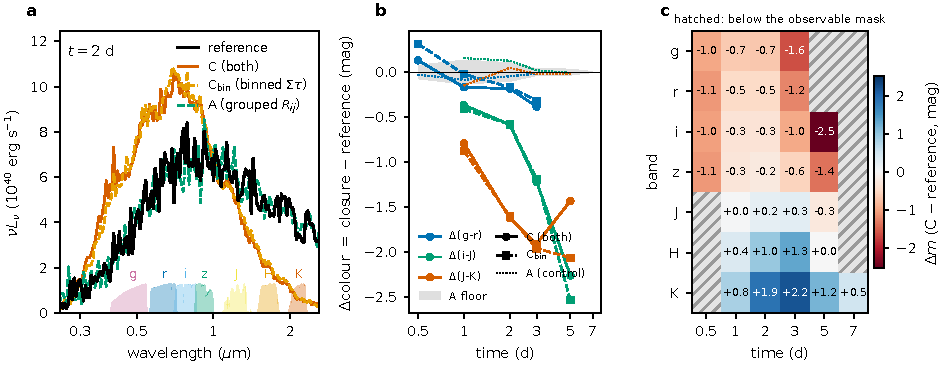
\includegraphics[width=\textwidth]{fig1_one_kilonova}
\caption{\textbf{The closure error on one kilonova.} The central model ($\Mej=0.01\,\Msun$, $\vej=0.1c$, $\Xlan=10^{-2}$). \textbf{a}, Emergent spectra at 2~d for the reference, the practical closure \Cboth, its exact-sum variant \Cbin and the redistribution-only control \Aleg; the DECam and 2MASS passbands are shaded. \textbf{b}, Colour differences from the reference through the six epochs for \Cboth (solid), \Cbin (dashed) and \Aleg (dotted); the grey band is the per-cell noise floor, the largest per-band \Aleg error. \textbf{c}, Per-band closure error of \Cboth; hatched cells fall below the observable mask.}
\label{fig:one}
\end{figure}

\begin{figure}[p]
\centering
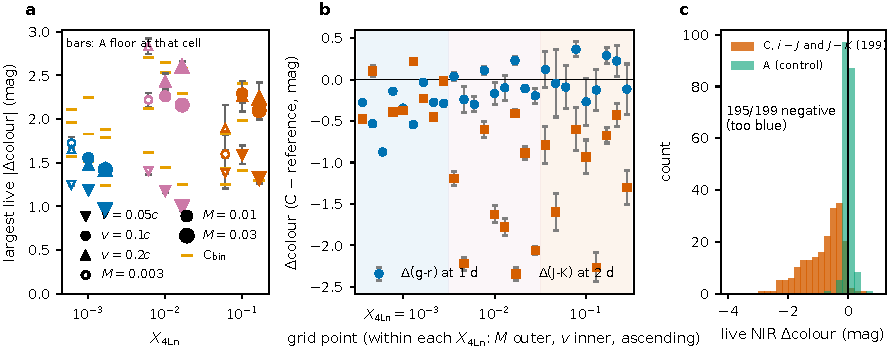
\includegraphics[width=\textwidth]{fig2_grid}
\caption{\textbf{Across the grid.} \textbf{a}, Largest live colour error per model for \Cboth (symbols: velocity; size and fill: mass) with the noise floor of that cell as the error bar, and for \Cbin (dashes). \textbf{b}, $\Delta(g-r)$ at 1~d and $\Delta(J-K)$ at 2~d at every grid point, ordered by lanthanide fraction (shaded), then mass, then velocity. \textbf{c}, The live near-infrared colour errors of \Cboth and of the control.}
\label{fig:grid}
\end{figure}

\begin{figure}[p]
\centering
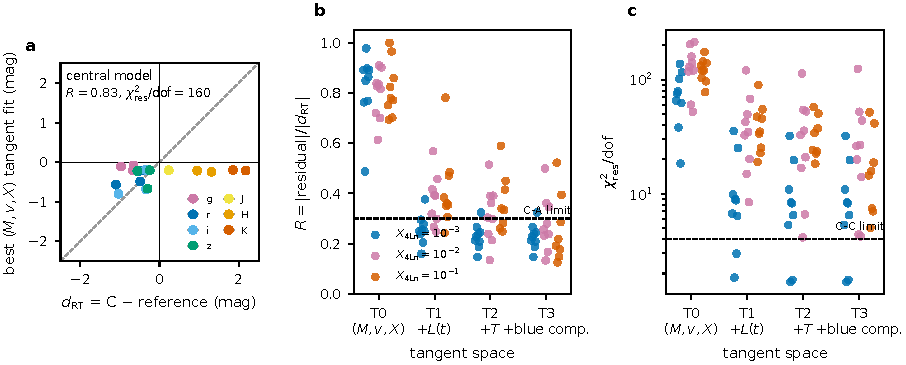
\includegraphics[width=\textwidth]{fig3_not_parameters}
\caption{\textbf{Not a parameter shift.} \textbf{a}, Closure error against its best fit in the $(\ln\Mej,\ln\vej,\ln\Xlan)$ tangent space at the central model, one point per live band and epoch; the fit has almost no projection on the error. \textbf{b}, Residual fraction $R$ per grid point under the ejecta parameters alone (T0) and with a free luminosity history (T1), a free colour temperature (T2) or a free blue second component (T3); the dashed line is the C-A limit. \textbf{c}, The same for $\chires$; the dashed line is the C-C limit.}
\label{fig:notparam}
\end{figure}

\begin{figure}[p]
\centering
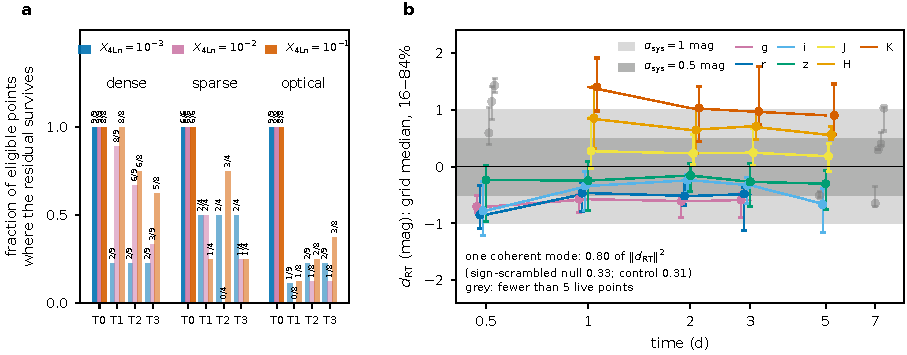
\includegraphics[width=\textwidth]{fig4_observability_syserr}
\caption{\textbf{Observability and structure.} \textbf{a}, Fraction of eligible grid points at \Distance\ Mpc where the closure residual is detected and survives the fit, per scenario and tangent space, by lanthanide fraction (counts above the bars). \textbf{b}, The closure error of \Cboth per band and epoch: grid median and 16--84\% range over the live points, against the $0.5$ and $1$~mag systematic allowances used in kilonova inference; keys with fewer than five live points are greyed.}
\label{fig:observe}
\end{figure}

\begin{table}[p]
\centering
\caption{\textbf{The verdict per lanthanide fraction.} Largest live colour error of \Cboth over the nine models at each $\Xlan$; the median noise floor of the well-sampled cells; grid points where the residual is structured (class C-B) under the ejecta parameters (Gate~2) and with a free luminosity history, with the median $\chires$ of the latter; and points where the residual survives observation at \Distance\ Mpc (Gate~3) under the three scenarios and, for the dense one, with the free luminosity history.}
\label{tab:verdict}
\footnotesize
\begin{tabular}{lccccccccc}
\toprule
$X_{\rm lan}$ & $|\Delta({\rm colour})|_{\max}$ & floor & Gate 2 & \multicolumn{2}{c}{free $L(t)$} & \multicolumn{3}{c}{Gate 3, $(M,v,X)$} & Gate 3, free $L(t)$ \\
 & (mag) & (mag) & C-B & C-B & $\chi^2_{\rm res}/{\rm dof}$ & dense & sparse & optical & dense \\
\midrule
$10^{-3}$ & 1.0--1.7 & 0.018 & 9/9 & 1/9 & 9 & 9/9 & 6/6 & 9/9 & 2/9 \\
$10^{-2}$ & 1.0--2.8 & 0.040 & 9/9 & 6/9 & 35 & 9/9 & 6/6 & 8/8 & 8/9 \\
$10^{-1}$ & 1.3--2.3 & 0.096 & 9/9 & 9/9 & 35 & 8/8 & 6/6 & 8/8 & 8/8 \\
\bottomrule
\end{tabular}

\end{table}

\clearpage
% ------------------------------------------------------------------ Methods
\section*{Methods}\label{sec:methods}
\addcontentsline{toc}{section}{Methods}

\subsection*{Transport code and reference}
The transport code is the vectorized Monte Carlo of Paper~II. Packets are launched from an inner boundary at radius $r_{\rm core}$ with a Planck spectrum at temperature $t_{\rm core}$ into a homologously expanding shell out to $r_{\rm out}$ at time $t_{\rm exp}$, and propagate under worldline (fully relativistic in $v/c$ to the order needed at $0.2c$) homologous kinematics: the comoving frequency decreases monotonically along every ray, so the next line a packet can meet is found by one search. In the reference mode a packet interacts with a line of Sobolev optical depth $\tau$ with probability $1-e^{-\tau}$; on interaction the pumped upper level decays through one of its radiative channels with probability proportional to the Einstein $A$ coefficient times that line's Sobolev escape probability $\beta=(1-e^{-\tau})/\tau$, and a packet that does not escape its emitting line is re-absorbed by it and draws again. Re-emission is isotropic in the comoving frame. A packet still in that re-absorption chain after \ChainBase\ links is thermalized in place and counted (\emph{trapped}); the grid caps the step count of the slowest packet at $10^6$, and no cell aborted.

\subsection*{The four closure legs}
Leg \Aleg (\texttt{sobolev\_group}) keeps the line-by-line Sobolev opacity and replaces the cascade by a $32$-group redistribution kernel $\Rij$: the probability that a packet absorbed in frequency group $i$ leaves through group $j$, with the exit frequency drawn from the discrete line frequencies inside $j$ so that the transport's at-resonance skip of the emitting line is preserved. The kernel is built at each epoch from the absorption--emission pairs of the reference run at that epoch, so it contains no information the reference does not, and no information the reference does. Leg \Bleg (\texttt{expansion\_branch}) replaces the line list by an expansion opacity on comoving bins of $\Delta\nu/\nu=4.17\times10^{-5}$ ($12.5$~km\,s$^{-1}$), the bin opacity being $\sum_k(1-e^{-\tau_k})$ over the lines it contains; on interaction the absorbing line is drawn within the bin with weight $1-e^{-\tau_k}$ and the packet exits through the reference's exact $A\beta$ kernel. Leg \Cboth (\texttt{expansion\_group}) combines the expansion opacity with the grouped kernel. Leg \Cbin (\texttt{binned\_group}) is \Cboth with the bin opacity $\sum_k\tau_k$ instead of $\sum_k(1-e^{-\tau_k})$. Lines with $\tau<10^{-3}$ are dropped from every leg alike. Each leg runs three seeds at the same packet count as the reference; all quantities are seed means.

\subsection*{Atoms}
The shell contains \LaII, \CeII, \PrII and \NdII with the lanthanide mass fraction $\Xlan$ split equally between them; the lanthanide fraction sets the line opacity of the shell and is otherwise a tracer (the diffusion opacity below is fixed). Level energies and transition probabilities are the calibrated tables of the atomic database of ref.~\cite{gsi_atomic} as distributed in ref.~\cite{gsi_zenodo}; the ions are treated as singly ionized with populations in local thermodynamic equilibrium at the gas temperature, with stimulated emission included in the line optical depths, and without radiative coupling between ions. No atomic quantity was adjusted.

\subsection*{Source model}
The ejecta are a uniform sphere of mass $\Mej$ expanding homologously to $\vej$. The heating rate per unit mass is the analytic r-process form $\dot\epsilon(t)=4\times10^{18}\,[\tfrac12-\pi^{-1}\arctan((t-t_0)/\sigma)]^{1.3}$~erg\,g$^{-1}$\,s$^{-1}$ of ref.~\cite{korobkin2012}, multiplied by the thermalization efficiency of ref.~\cite{barnes2016} interpolated bilinearly in $(\log\Mej,\vej)$. The bolometric luminosity is the one-zone diffusion solution of ref.~\cite{arnett1982} with a fixed grey opacity $\kappa=1$~cm$^2$\,g$^{-1}$, so that the light curve depends on $(\Mej,\vej)$ and not on $\Xlan$. The photosphere is the grey $\tau=2/3$ surface, $v_{\rm ph}/\vej = 1-\tfrac{2}{3}/(\kappa\rho\vej t)$, floored at $v_{\rm ph}/\vej=0.5$ and flagged where the floor binds; the packets are launched from it with the blackbody temperature $\Teff=[L/(4\pi\sigma R_{\rm ph}^2)]^{1/4}$, and the gas temperature of the shell is set equal to $\Teff$. Every epoch is an independent snapshot. On the central model $\Teff$ falls from $\sim9700$~K at $0.5$~d to $\sim1800$~K at $7$~d (Extended Data Fig.~\ref{edfig:source}).  % literal-ok

\subsection*{Grid, budgets and noise floor}
The \nModels\ models were run at six epochs with $n=3\times10^5$ packets per seed and per leg, scaled down per epoch to a $1500$~s wall-clock budget for the reference (floor $2\times10^4$); nine cells whose floor would have exceeded three times the budget were run afterwards at a $5400$~s budget, so that the grid is \nCellsRan\ of \nCells\ cells. The Monte Carlo noise floor of a cell is the largest per-band error of leg \Aleg at that cell, which is a redistribution-only closure whose error is expected to be at the noise level; its statistics are quoted from the \FloorNWell\ cells with $n\ge10^5$ per seed. Twenty-seven epoch rows in twelve models have the photosphere at its floor and are excluded from every derivative-based comparison. Floored-photosphere epochs were excluded from derivative-based comparisons, all headline results were regenerated after this mask was enforced, and classifications were unchanged for points evaluable under both definitions.

\subsection*{Photometry and normalization}
Spectra are accumulated on 200 logarithmic frequency bins between $1000$ and $30000$~\AA\ and integrated through the DECam $g,r,i,z$ and 2MASS $J,H,K_s$ transmission curves \cite{flaugher2015,skrutskie2006} as distributed by the SVO Filter Profile Service \cite{svofps2012,svofps2024}, in the AB system at \Distance\ Mpc. Because the cascade changes a packet's energy by the level-energy difference at every fluorescence, the branching Monte Carlo conserves photon number, not energy, and at hundreds of interactions per packet the escaped energy is not a prediction of the bolometric luminosity. Every leg is therefore normalized so that its escaped energy inside the window equals the source luminosity (\emph{conserving} core): $\Delta m_{\rm bol}\equiv0$ by construction, and the closure error is a colour. The absorbing- and equilibrium-core normalizations are stored alongside; colours are identical under all three, as each is a grey rescaling.

\subsection*{Observable mask}
An observable $(b,t)$ is live at a grid point if the reference band luminosity is at least $1\%$ of the bolometric luminosity, the reference magnitude is brighter than $23.5$ (optical) or $21.5$ (near-infrared), and the epoch is not floored. The observational errors used in the parameter-fit test are $\sigma=0.05$~mag optical and $0.10$~mag near-infrared. The mask is applied to the reference alone, so that every leg is compared on the same observables, and the number of live observables per grid point (Extended Data Table~\ref{edtab:grid}) is set by the epoch at which each band drops below the depth or the luminosity share.  % literal-ok

\subsection*{Parameter-fit test (Gate 2)}
At each grid point the derivatives $\partial m_b(t)/\partial\ln\theta$ for $\theta\in(\Mej,\vej,\Xlan)$ are central differences of the reference photometry across the grid (one-sided at the edges; the $\Xlan$ secant spans one decade), on the intersection of the live masks. A derivative component smaller than three times the noise floor propagated through the finite difference is set to zero. The closure error $\dRT$ is fitted by weighted least squares, $\dRT\approx D\,a$, with $\sigma$ as above; $R=\|\dRT-Da\|_\sigma/\|\dRT\|_\sigma$, $\chires$ with ${\rm dof}=N-{\rm rank}(D)$, and a point is \emph{underdetermined} if ${\rm dof}<4$. Class C-C: $\chi^2_{\rm RT}/N\le\ThrChi$. Class C-A: $R\le\ThrR$ and some physical $|a_\theta|\ge\ThrSignif\,\sigma_{a_\theta}$. Class C-B otherwise. The nuisance spaces add columns: T1, a grey offset per epoch with at least two live observables; T2, the Planck derivative $\partial m_b/\partial\ln T$ at fixed luminosity evaluated at the row's $\Teff$; T3, a linearized blue second component whose photometry is that of the same-$(\Mej,\vej)$ model at $\Xlan=10^{-3}$, with the fitted amplitude reported against the linearization. Chain-cap sensitivity is tested by replacing the four highest-trapped cells with their \ChainTop-cap results and re-running the classification.

\subsection*{Observing scenarios (Gate 3)}
Each live observable receives an error $\sigma(m)=[\sigsys^2+(1.0857/{\rm SNR})^2]^{1/2}$ with ${\rm SNR}=5\times10^{-0.4(m-m_{5\sigma})}$, $\sigsys=0.03$ (optical) and $0.05$ (near-infrared). Dense: $griz$ and $JHK_s$ at all six epochs to $m_{5\sigma}=23.5$ and $21.5$. Sparse: $griz$ at 1, 3 and 7~d, $JHK_s$ at 2 and 5~d, to $22.5$ and $20.5$. Optical: $griz$ at all six epochs, no near-infrared. A point is eligible with at least eight observations; it survives if $\chi^2_{\rm RT}/N\ge\ThrChi$ under the scenario's errors and the fit leaves class C-B. The near-infrared share is the fraction of $\chi^2_{\rm RT}$ carried by $JHK_s$.

\subsection*{Temperature-direction validation}
At the central point the reference was re-run with the launch temperature scaled by $0.8$ and $1.25$ at fixed luminosity and photospheric radius, once changing only the illuminating spectrum and once changing the gas temperature with it. The Monte Carlo temperature direction $d_T=[m(1.25)-m(0.8)+2.5\log_{10}(L_{1.25}/L_{0.8})]/\ln1.5625$ is compared with the Planck proxy on the live observables by a $1/\sigma^2$-weighted cosine and norm ratio (Extended Data Fig.~\ref{edfig:tscale}). The central point remains class C-B under either version of the T2 column.

\subsection*{The allowance comparison}
The $\nPoints\times\SysKeys$ matrix of $\dRT$ (points by band--epoch keys) is analysed unweighted, in magnitudes, on its live entries. The one-mode fraction is a masked rank-one fit $X\approx uv^{\mathsf T}$ by alternating least squares on the observed entries, $f_1=1-\sum(X-uv^{\mathsf T})^2/\sum X^2$; the cross-check is a singular-value decomposition of the median-filled matrix restricted to keys live at ten or more points. The null is the same statistic on the same entries with independently scrambled signs (fixed seed, 1000 draws), which preserves amplitude and mask and destroys coherence; the Marchenko--Pastur expectation for an independent matrix of this shape is \SysMPScale. The $\chi^2$-equivalent is $\sum(\dRT/\sigsys)^2/N$ per point.

\subsection*{Data availability}
Every number in this paper is generated from \texttt{paper3/FROZEN.json} in the repository, which records the SHA-256 of every transport output, every derived table and every figure, together with the commit and the tree hashes of the input directories; the tag \texttt{paper3-freeze} marks the state the manuscript was built from.

\subsection*{Code availability}
The transport code, the source model, the grid drivers, the analysis and the manuscript generators are in the public repository accompanying Papers~I--III \todo{repository URL}. \texttt{python paper3/freeze.py --check --strict} regenerates every derived quantity and figure and compares them to the frozen record; the test suite runs with \texttt{pytest}.

\clearpage
\section*{Extended Data}\label{sec:ed}
\setcounter{figure}{0}\renewcommand{\figurename}{Extended Data Fig.}
\setcounter{table}{0}\renewcommand{\tablename}{Extended Data Table}

\begin{figure}[h]
\centering
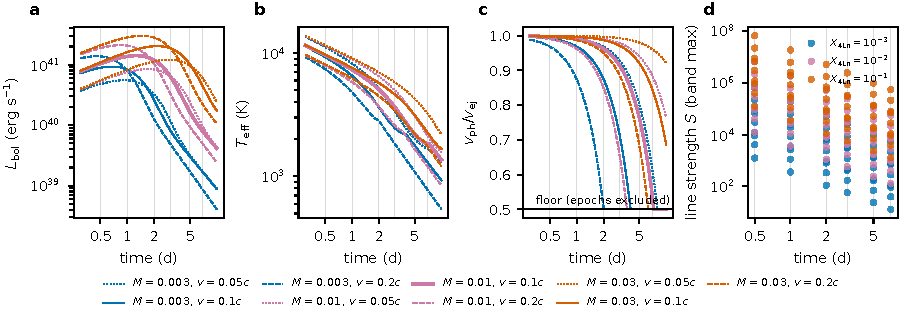
\includegraphics[width=\textwidth]{edfig1_source}
\caption{\textbf{The source model and its gate.} \textbf{a}--\textbf{c}, Bolometric luminosity, photospheric temperature and photospheric velocity fraction of the nine $(\Mej,\vej)$ combinations; the floor at $v_{\rm ph}/\vej=0.5$ marks the epochs excluded from derivative-based comparisons. \textbf{d}, Band line strength $S$ (maximum over bands of the line optical depth per velocity bin) of every ran cell.}
\label{edfig:source}
\end{figure}

\begin{figure}[h]
\centering
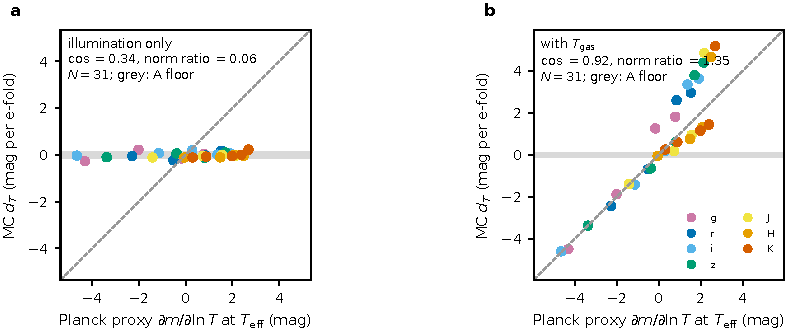
\includegraphics[width=\textwidth]{edfig2_tscale}
\caption{\textbf{The temperature direction.} Monte Carlo derivative of the reference photometry with respect to $\ln T$ at the central point against the Planck proxy at $\Teff$, when only the illuminating spectrum is scaled (\textbf{a}) and when the gas temperature is scaled with it (\textbf{b}); the grey band is the noise floor.}
\label{edfig:tscale}
\end{figure}

\begin{figure}[h]
\centering
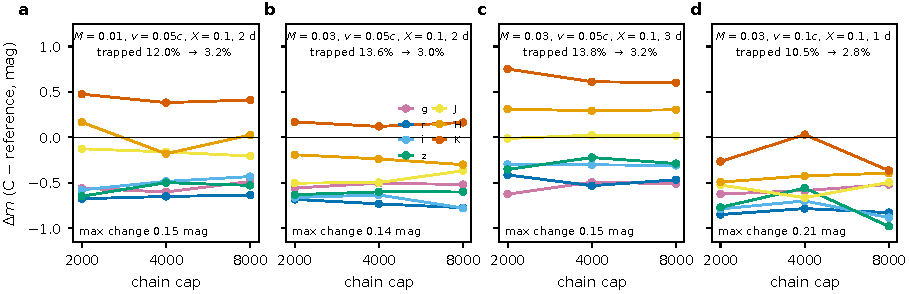
\includegraphics[width=\textwidth]{edfig3_chain_cap}
\caption{\textbf{The chain cap.} Per-band closure error of \Cboth at the four cells with the highest trapped fraction, for re-absorption caps of \ChainBase, 4000 and \ChainTop\ links; the trapped fraction at the base and top caps is given in each panel.}
\label{edfig:chain}
\end{figure}

\begin{figure}[h]
\centering
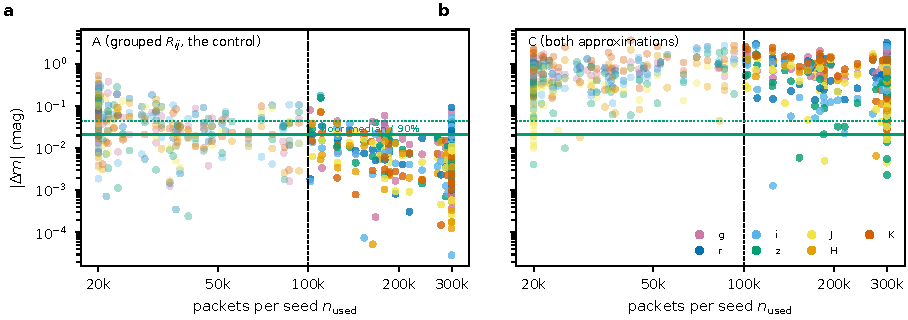
\includegraphics[width=\textwidth]{edfig4_control_floor}
\caption{\textbf{The control across the grid.} Absolute per-band error of the redistribution-only control \Aleg (\textbf{a}) and of \Cboth (\textbf{b}) at every live observable against the packet count of the cell; the dashed line is the well-sampled threshold and the horizontal lines the median and 90th percentile of the noise floor.}
\label{edfig:control}
\end{figure}

\begin{table}[h]
\centering
\caption{\textbf{The grid.} Per model: live observables $N$, packets per seed, largest trapped fraction, largest well-sampled noise floor, largest live colour error of \Cboth and \Cbin with the colour and, under the four tangent spaces, the class.}
\label{edtab:grid}
\small
\resizebox{\textwidth}{!}{\begin{tabular}{cccrcrrcccccc}
\toprule
$M_{\rm ej}$ & $v_{\rm ej}$ & $X_{\rm lan}$ & $N$ & $n_{\rm used}$ & trapped & floor & $|\Delta{\rm col}|_{\max}$ & $|\Delta{\rm col}|_{\max}$ & \multicolumn{4}{c}{class} \\
($M_\odot$) & ($c$) & & & ($10^3$) & (\%) & (mag) & C & C$_{\rm bin}$ & T0 & T1 & T2 & T3 \\
\midrule
0.003 & 0.05 & $10^{-3}$ & 20 & 186--300 & 0.0 & 0.032 & 1.25 (i-J) & 1.57 (i-J) & C-B & C-A & C-B & C-B \\
0.003 & 0.05 & $10^{-2}$ & 17 & 35--300 & 1.2 & 0.039 & 1.40 (J-K) & 1.62 (J-K) & C-B & C-B & C-B & C-A \\
0.003 & 0.05 & $10^{-1}$ & 17 & 20--176 & 8.9 & -- & 1.38 (J-K) & 1.25 (J-K) & C-B & C-B & C-A & C-A \\
0.003 & 0.1 & $10^{-3}$ & 11 & 144--300 & 0.0 & 0.070 & 1.72 (i-J) & 2.11 (i-J) & C-B & C-A & C-B & C-B \\
0.003 & 0.1 & $10^{-2}$ & 10 & 21--300 & 1.0 & 0.081 & 2.22 (J-K) & 2.12 (J-K) & C-B & C-B & C-A & C-A \\
0.003 & 0.1 & $10^{-1}$ & 7 & 20--300 & 8.2 & -- & 1.60 (J-K) & 1.44 (J-K) & C-B & C-B & underdet. & underdet. \\
0.003 & 0.2 & $10^{-3}$ & 14 & 111--300 & 0.0 & 0.033 & 1.65 (i-J) & 1.96 (i-J) & C-B & C-A & C-A & C-A \\
0.003 & 0.2 & $10^{-2}$ & 13 & 20--300 & 0.1 & -- & 2.84 (J-K) & 2.71 (J-K) & C-B & C-B & C-B & C-B \\
0.003 & 0.2 & $10^{-1}$ & 11 & 20--300 & 5.6 & -- & 1.90 (J-K) & 1.84 (J-K) & C-B & C-B & C-B & C-B \\
0.01 & 0.05 & $10^{-3}$ & 21 & 217--300 & 0.1 & 0.025 & 1.19 (i-J) & 1.51 (i-J) & C-B & C-A & C-B & C-B \\
0.01 & 0.05 & $10^{-2}$ & 20 & 32--300 & 1.2 & 0.026 & 1.18 (J-K) & 1.44 (J-K) & C-B & C-A & C-A & C-A \\
0.01 & 0.05 & $10^{-1}$ & 20 & 20--83 & 12.0 & -- & 1.59 (J-K) & 1.41 (J-K) & C-B & C-B & C-B & C-A \\
0.01 & 0.1 & $10^{-3}$ & 21 & 173--300 & 0.0 & 0.027 & 1.55 (i-J) & 2.24 (i-J) & C-B & C-A & C-A & C-A \\
0.01 & 0.1 & $10^{-2}$ & 17 & 24--300 & 0.9 & 0.039 & 2.26 (i-J) & 2.53 (i-J) & C-B & C-B & C-B & C-B \\
0.01 & 0.1 & $10^{-1}$ & 17 & 20--162 & 9.0 & 0.014 & 2.29 (J-K) & 2.41 (J-K) & C-B & C-B & C-A & C-A \\
0.01 & 0.2 & $10^{-3}$ & 14 & 125--300 & 0.0 & 0.034 & 1.47 (i-J) & 1.83 (i-J) & C-B & C-A & C-A & C-A \\
0.01 & 0.2 & $10^{-2}$ & 11 & 20--300 & 0.8 & 0.092 & 2.43 (i-J) & 2.65 (J-K) & C-B & C-B & C-B & C-A \\
0.01 & 0.2 & $10^{-1}$ & 11 & 20--300 & 6.6 & -- & 2.26 (J-K) & 1.98 (J-K) & C-B & C-B & C-B & C-A \\
0.03 & 0.05 & $10^{-3}$ & 34 & 300--300 & 0.1 & 0.016 & 0.96 (i-J) & 1.24 (i-J) & C-B & C-A & C-A & C-A \\
0.03 & 0.05 & $10^{-2}$ & 30 & 37--167 & 1.4 & 0.043 & 0.99 (J-K) & 1.26 (J-K) & C-B & C-A & C-A & C-A \\
0.03 & 0.05 & $10^{-1}$ & 30 & 20--45 & 13.8 & -- & 1.32 (J-K) & 1.30 (J-K) & C-B & C-B & C-B & C-B \\
0.03 & 0.1 & $10^{-3}$ & 30 & 206--300 & 0.1 & 0.023 & 1.42 (i-J) & 1.88 (i-J) & C-B & C-A & C-A & C-A \\
0.03 & 0.1 & $10^{-2}$ & 29 & 31--300 & 1.2 & 0.059 & 2.16 (i-J) & 2.30 (i-J) & C-B & C-A & C-A & C-A \\
0.03 & 0.1 & $10^{-1}$ & 26 & 20--76 & 10.5 & -- & 2.10 (J-K) & 2.07 (J-K) & C-B & C-B & C-B & C-A \\
0.03 & 0.2 & $10^{-3}$ & 26 & 180--300 & 0.0 & 0.034 & 1.42 (i-J) & 1.79 (i-J) & C-B & C-B & C-B & C-B \\
0.03 & 0.2 & $10^{-2}$ & 24 & 23--300 & 1.1 & 0.054 & 2.60 (i-J) & 2.58 (i-J) & C-B & C-B & C-B & C-B \\
0.03 & 0.2 & $10^{-1}$ & 23 & 20--263 & 8.4 & 0.178 & 2.24 (J-K) & 2.12 (J-K) & C-B & C-B & C-B & C-B \\
\bottomrule
\end{tabular}
}
\end{table}

\begin{table}[h]
\centering
\caption{\textbf{Observing scenarios and Gate 3.} Epochs, $5\sigma$ depths and photometric systematics of the three scenarios, and the eligible and surviving points under the four tangent spaces.}
\label{edtab:scenarios}
\small
\resizebox{\textwidth}{!}{\begin{tabular}{llcccccc}
\toprule
scenario & epochs (d) & depth & $\sigma_{\rm sys}$ & \multicolumn{4}{c}{eligible / survives} \\
 & optical; NIR & opt / NIR & opt / NIR & T0 & T1 & T2 & T3 \\
\midrule
dense & 0.5, 1, 2, 3, 5, 7; 0.5, 1, 2, 3, 5, 7 & 23.5 / 21.5 & 0.03 / 0.05 & 26 / 26 & 26 / 18 & 26 / 14 & 26 / 10 \\
sparse & 1, 3, 7; 2, 5 & 22.5 / 20.5 & 0.03 / 0.05 & 18 / 18 & 12 / 5 & 12 / 5 & 12 / 4 \\
optical & 0.5, 1, 2, 3, 5, 7; -- & 23.5 / -- & 0.03 / -- & 25 / 25 & 25 / 2 & 25 / 5 & 25 / 6 \\
\bottomrule
\end{tabular}
}
\end{table}

\clearpage
\bibliographystyle{unsrtnat}
\bibliography{references}
\end{document}
